% \documentclass[12pt, border = 8pt, varwidth, convert]{standalone}
\documentclass[margin=3pt,
   varwidth, 
  convert,
  convert={
    outext=.png,
    command=\unexpanded{
      pdftocairo -r 300 -png \infile % 将生成的pdf文件转换为png图像
    }
  }
  ]{standalone}

\usepackage{tkz-fct}

\begin{document} %在document环境中撰写文档
% \begin{tikzpicture}
%   % 定义坐标区域
%   \tkzInit[xmin=0, xmax=6, ymin=0, ymax=6]
%   % 绘制坐标轴
%   \tkzDrawXY[>=stealth']
%   % 绘制曲线
%   \tkzFct[thick,color=red, domain=0:6]{5*sin(x)}% 曲线a
%   \tkzFct[thick,color=blue, domain=0:3]{x**2}% 曲线b
%   \tkzFct[thick,color=green, domain=0.2:5]{1.0/x}% 曲线c
%   \def\tkzFctgnud{0}% 曲线d
%   % 绘制填充区域
%   %\tkzDrawAreafg[pattern=north east lines, between= a and b, color=gray!80, domain = 0:pi]
%   \tkzDrawAreafg[pattern=dots, between= b and d, color=gray!50, domain = 0:1]
%   % \tkzDrawAreafg[pattern=dots, between= c and d, color=gray!50, domain = 1:5]
%   % \tkzDrawAreafg[pattern=bricks, between= b and c, color=gray!50,domain = 0:3]
%   % \tkzDrawAreafg[between= b and f,color=gray!80,domain = 8:18]
%   % \tkzDrawAreafg[between= d and c,color=gray!50,domain = 2:20]
% \end{tikzpicture}

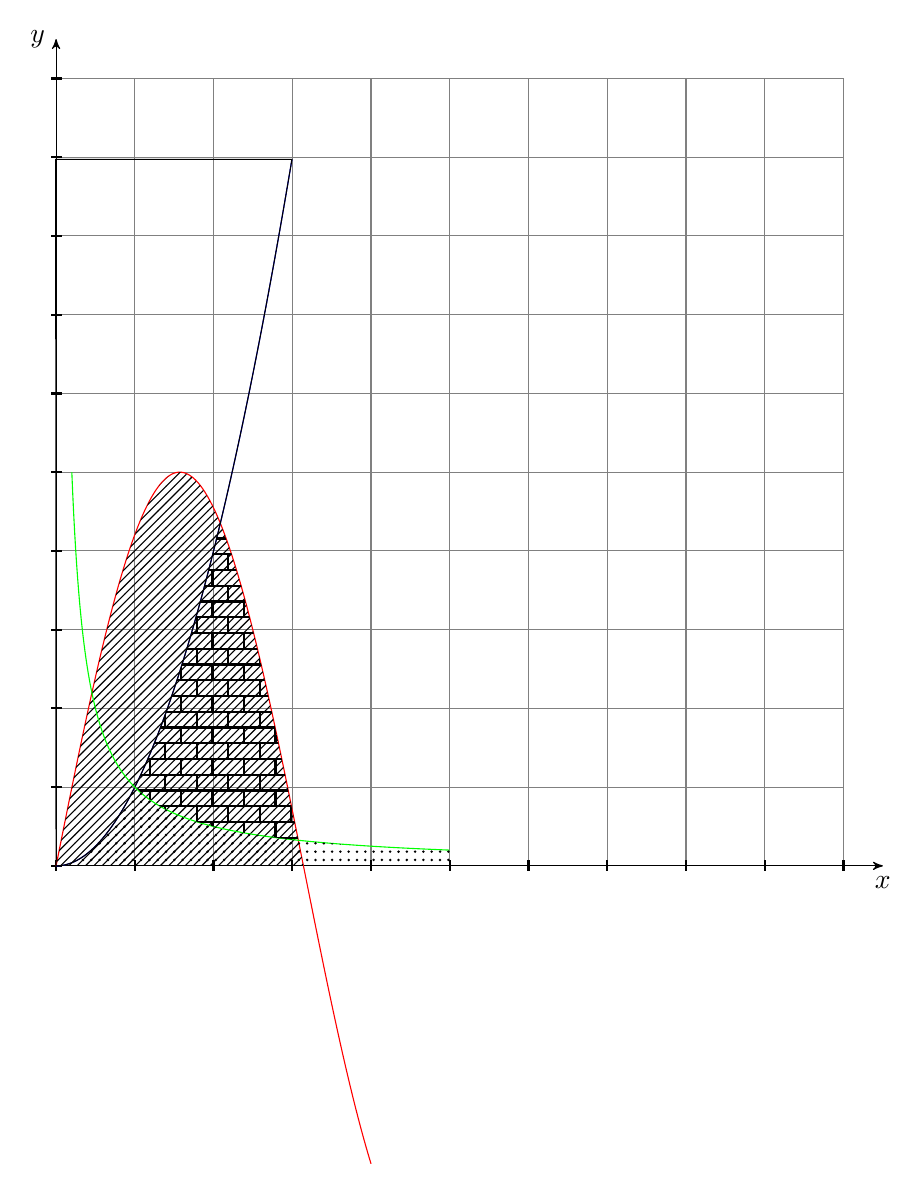
\begin{tikzpicture}[domain=0:4]
    \tkzGrid
    \tkzDrawXY[>=stealth']
    \draw[red] plot[samples=400](\x,{5*sin(\x r)});
    \draw[blue] plot[samples=400,domain=0:3](\x,{\x^2});
    \begin{scope}
        \draw plot[samples=400,domain=0:3](\x,{\x^2})--++(-3,0)--cycle;
        \path[pattern=north east lines] (0,0)--plot[domain=0:pi](\x,{5*sin(\x r)})--cycle;
    \end{scope}
    \draw[green] plot[samples=400,domain=0.2:5](\x,{1/\x});
    \begin{scope}
        \clip (0,0)plot[domain=0:2](\x,{\x^2})--(5,2)--(5,0)--cycle;
        \clip plot[domain=0.2:5](\x,{1/\x})--(5,0)--(0,0)--(0,5)--cycle;
        \path[pattern=dots] (0,0)rectangle(5,3);
    \end{scope}

    \begin{scope}
        \clip plot[domain=0:3](\x,{\x^2})--++(2,0)--(5,0)--cycle;
        \clip plot[domain=0.1:5](\x,{1/\x})--(5,5)--cycle;
        \clip plot[domain=0:pi](\x,{5*sin(\x r)})--(0,0);
        \path[pattern=bricks] (0,0)rectangle(5,5);
    \end{scope}
\end{tikzpicture}
% \begin{tikzpicture}[scale=.75]
%   \tkzInit[xmax=20,ymax=12]
%   \tkzGrid[color=orange,sub](0,0)(20,12)
%   \tkzAxeXY
%   \tkzFct[samples=400,domain =0:8]{(32-4*x)**(0.5)}% a
%   \tkzFct[samples=400,domain =0:18]{(72-4*x)**(0.5)}% b
%   \tkzFct[samples=400,domain =0:20]{(112-4*x)**(0.5)}% c
%   \tkzFct[samples=400,domain =2:20]{(152-4*x)**(0.5)}% d
%   \tkzFct[samples=400,domain =12:20]{(192-4*x)**(0.5)}% e
%   \def\tkzFctgnuf{0}% f
%   \def\tkzFctgnug{12}% g
%   % \tkzDrawAreafg[between= b and a,color=gray!80,domain = 0:8]
%   \tkzDrawAreafg[between= b and f,color=gray!80,domain = 8:18]
%   % \tkzDrawAreafg[between= d and c,color=gray!50,domain = 2:20]
%   \tkzDrawAreafg[between= g and c,color=gray!50,domain = 0:2]
%   % \tkzDrawAreafg[between= g and e,color=gray!20,domain =12:20]
% \end{tikzpicture}%
\end{document}

%%% Local Variables:
%%% mode: latex
%%% TeX-master: t
%%% End:
